
\paragraph{Label Propagation algorithm in Fault Free execution}

\begin{figure*}

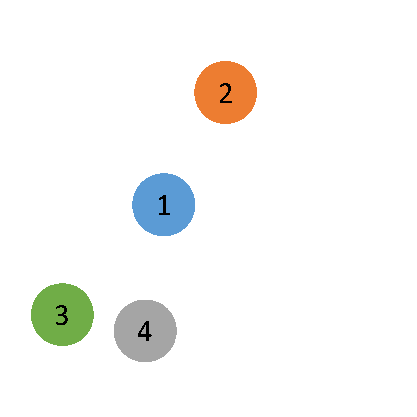
\includegraphics[width=0.2\paperwidth]{figure/sv1}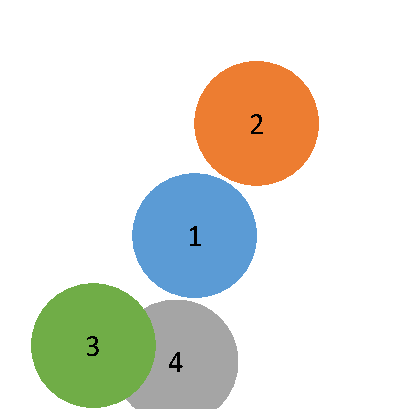
\includegraphics[width=0.2\paperwidth]{figure/sv2}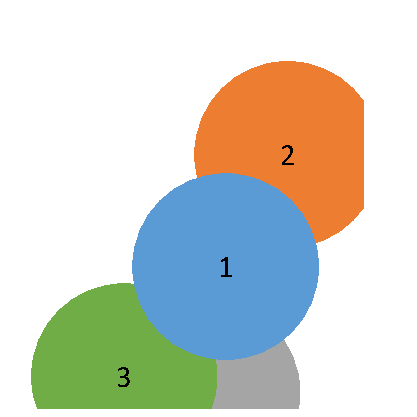
\includegraphics[width=0.2\paperwidth]{figure/sv3}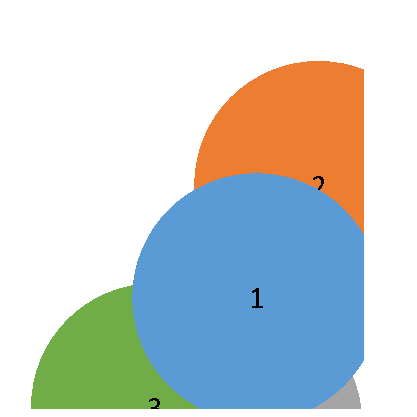
\includegraphics[width=0.2\paperwidth]{figure/sv4}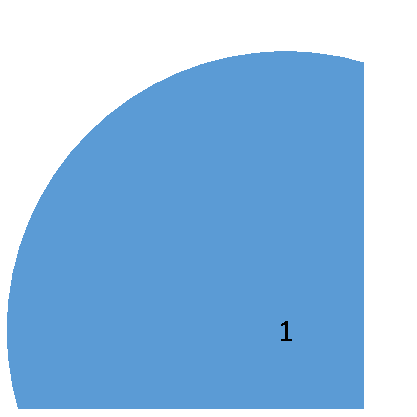
\includegraphics[width=0.2\paperwidth]{figure/sv5}\caption{These sub-figures conceptually show how the connected component id
propagates through the graph as time evolves. Subfigures represent
snapshots of the algorithm at different times. For simplicity, this
example assumes that all the shown vertices are connected. Initially
the number of connected components is equal to the number vertices.
(a) Depicts the initial state in which each vertex is in its own component.
(b)-(d) depict that some vertices belong to the same connected component
yet may require multiple label updates (in either the same iteration
or a separate iteration). (e) is the final state in which there is
a single connected component.}

\end{figure*}

\begin{table}

\centering
\footnotesize
\caption{Symbols used in the fault free \sv algorithm and in the new fault tolerant algorithm.}
\begin{tabular}[t]{|l|l|r|}\hline
Symbol & Decription & Size\\\hline\hline
$V$ & Vertices in the graph & O(V)\\\hline
$E$ & Edges in the graph & O(E)\\\hline
$adj(v)$ & Adjacency list for vertex $v\in V$ & \\\hline
\CCVAL & Connected component array & O(V)\\\hline
\CCVAL$^i$ & Connected component array after iteration $i$ & O(V)\\\hline
\CCVAL$^\infty$ & The final connected component mapping upon algorithm completion. & O(V)\\\hline

& Fault free \\
\hline
$H$ &  & O(V)\\\hline
\end{tabular}
\label{tab:symbols}

\end{table}

The aim of label propagation algorithm is to mark every vertex in
a given connected component with a pre-defined common label. This
common label is same within each connected component, and different
across different connected component. There are many choice for the
common label. As a convention, we consider minimum vertex-id in the
connected component as the final common label. 

The label propgation algorithm keeps an array $CC$ of current labels
for all vertices. For each vertex $v$, its label $CC[v]$ is initalized
with its vertex-id $CC[v]=v$. In every iteration, each vertex updates
its label by calculating minimum label of all its neighbours and itself:
\begin{equation}
CC^{i+1}[v]=\min_{u\in\mathcal{N}(v)}CC^{i}[u],\label{eq:lp_update_eqn}
\end{equation}

where $\mathcal{N}(v)=\left\{ v,adj(v)\right\} $ is the defined as
immidiate neighbourhood of $v$. Thus, through out the iteration minimum
vertex id propagates to all the vertces in the connect component.
The iteration converges when there are no more label changes in the
graph. 

Depending on the constrints, equation \ref{eq:lp_update_eqn} can
be implmented in two ways. In the first way, we use two different
arrays to store $CC^{i+1}$ and $CC^{i}$. We refer to this implementation
is Sync LP algorithm. In an another way, we overwrite $CC^{i+1}$
on $CC^{i}$. We refer to this version as Async LP algorithm. Depending
on architecture and programming model, the two variants may have different
performance characteristics. In subsequent discussion, we assume Async
LP algorithm. Yet, our results are equally applicable to both instance
of the LP algorithm.

Each iteration of LP, visits all the vertex and edges once and thus
costs $\mathcal{O}(V+E)$. The LP algorithm requires $\mathcal{O}(d)$
iterations to converge, where $d$ is the diameter of the graph. We
may use short-cutting to bound the number of iteration to $\mathcal{O}(log(d))$
{[}insert citation{]}. However, in practice async LP algorithm only
takes a few more iteration than implementing full short cutting step,
without the cost of short cutting. 
